\chapter{Web Dashboard Interface} \label{app:web_dashboard}

This appendix presents the UAchado web dashboard interface used by local managers and system administrators. The dashboard enables oversight of lost and found operations through analytical panels and management interfaces.

\begin{figure}[h]
    \centering
    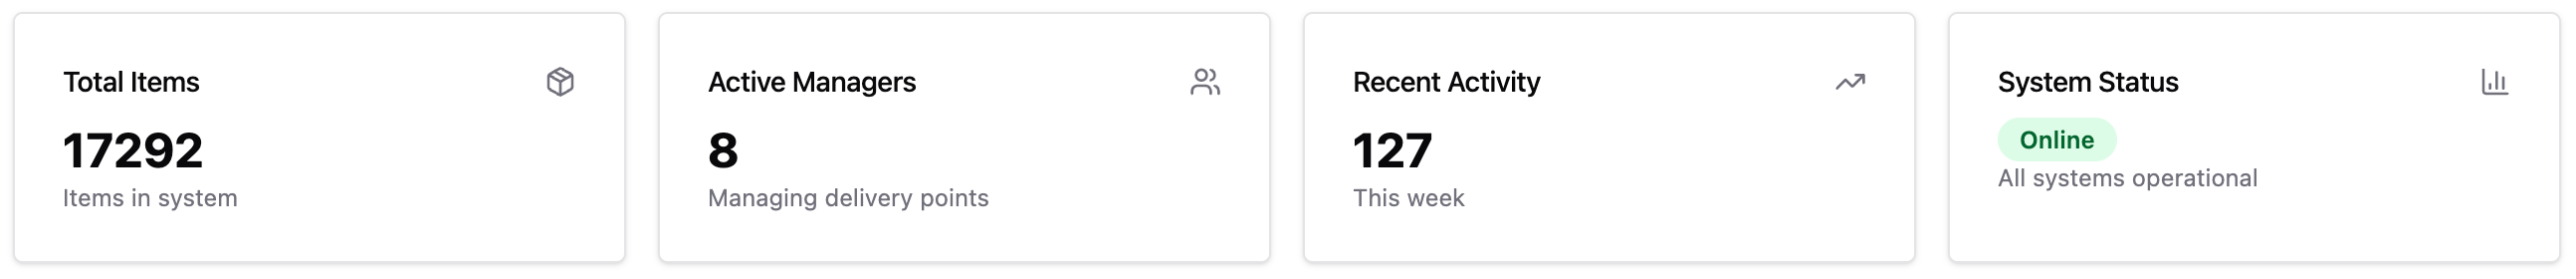
\includegraphics[width=\textwidth]{figs/appendix/web/1.png}
    \caption{System overview dashboard displaying key performance indicators including total items, active managers, recent weekly activities, and overall system status.}
    \label{fig:web_dashboard_overview}
\end{figure}

\begin{figure}[h]
    \centering
    \begin{subfigure}[b]{0.32\textwidth}
        \centering
        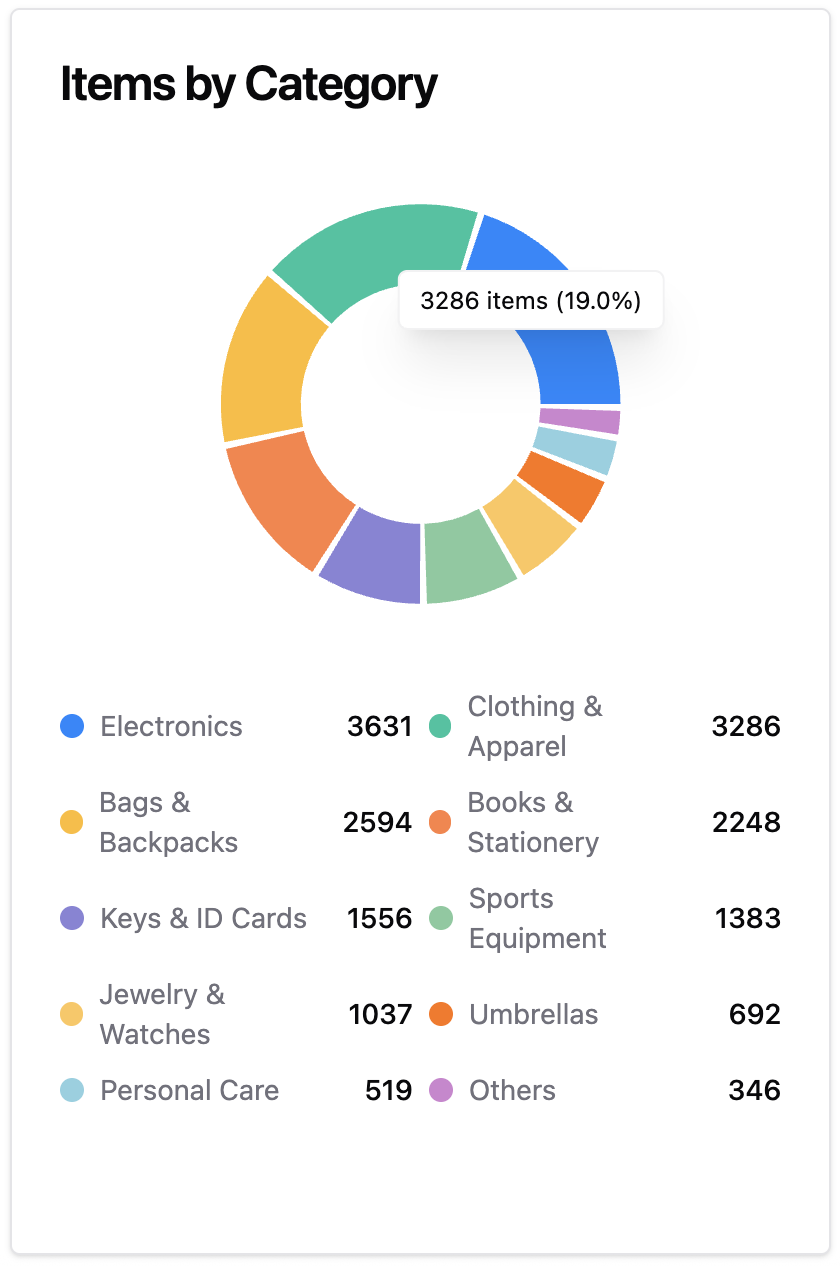
\includegraphics[width=\textwidth]{figs/appendix/web/2A.png}
        \caption{Items by category distribution showing Electronics as the largest category, followed by Clothing \& Apparel and other categories.}
        \label{fig:web_items_category}
    \end{subfigure}
    \hfill
    \begin{subfigure}[b]{0.32\textwidth}
        \centering
        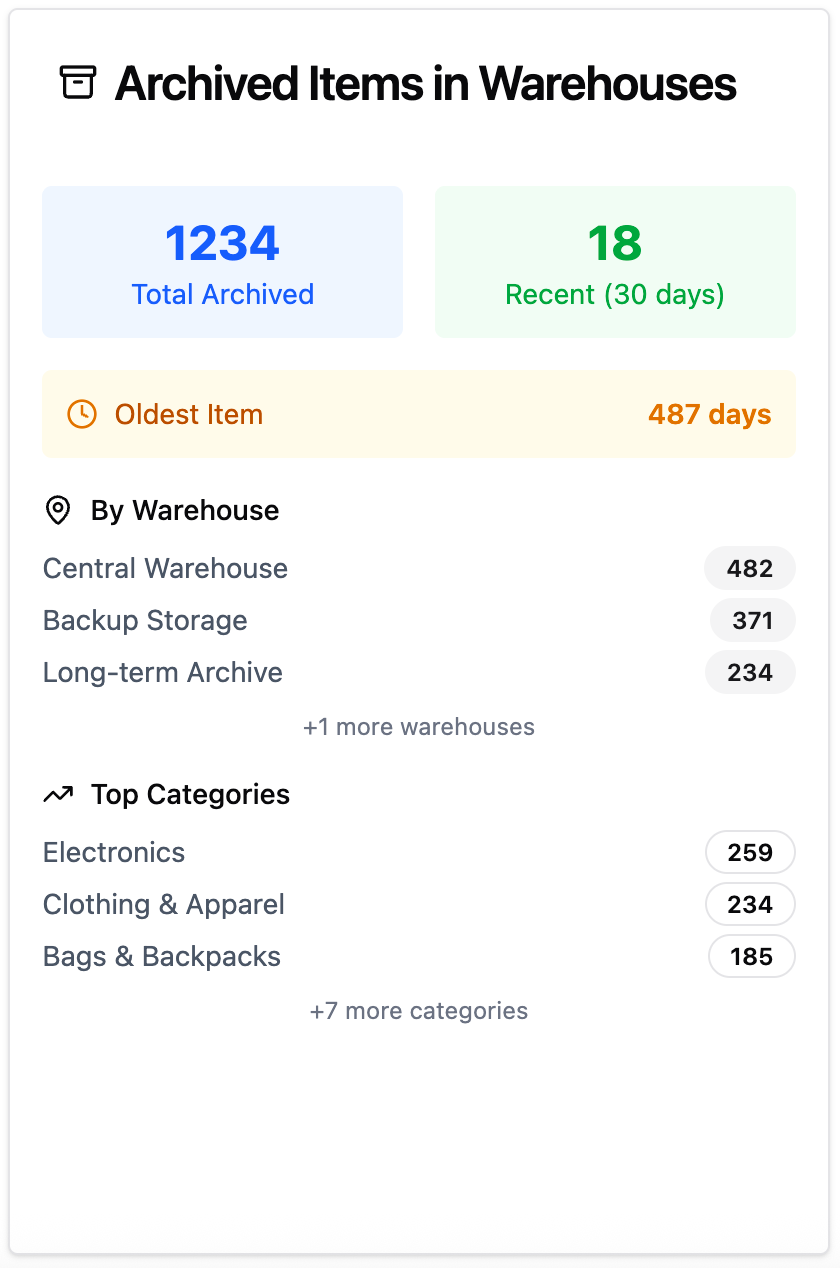
\includegraphics[width=\textwidth]{figs/appendix/web/2B.png}
        \caption{Archived items in warehouses overview displaying 1,234 total archived items distributed across multiple storage facilities.}
        \label{fig:web_archived_items}
    \end{subfigure}
    \hfill
    \begin{subfigure}[b]{0.32\textwidth}
        \centering
        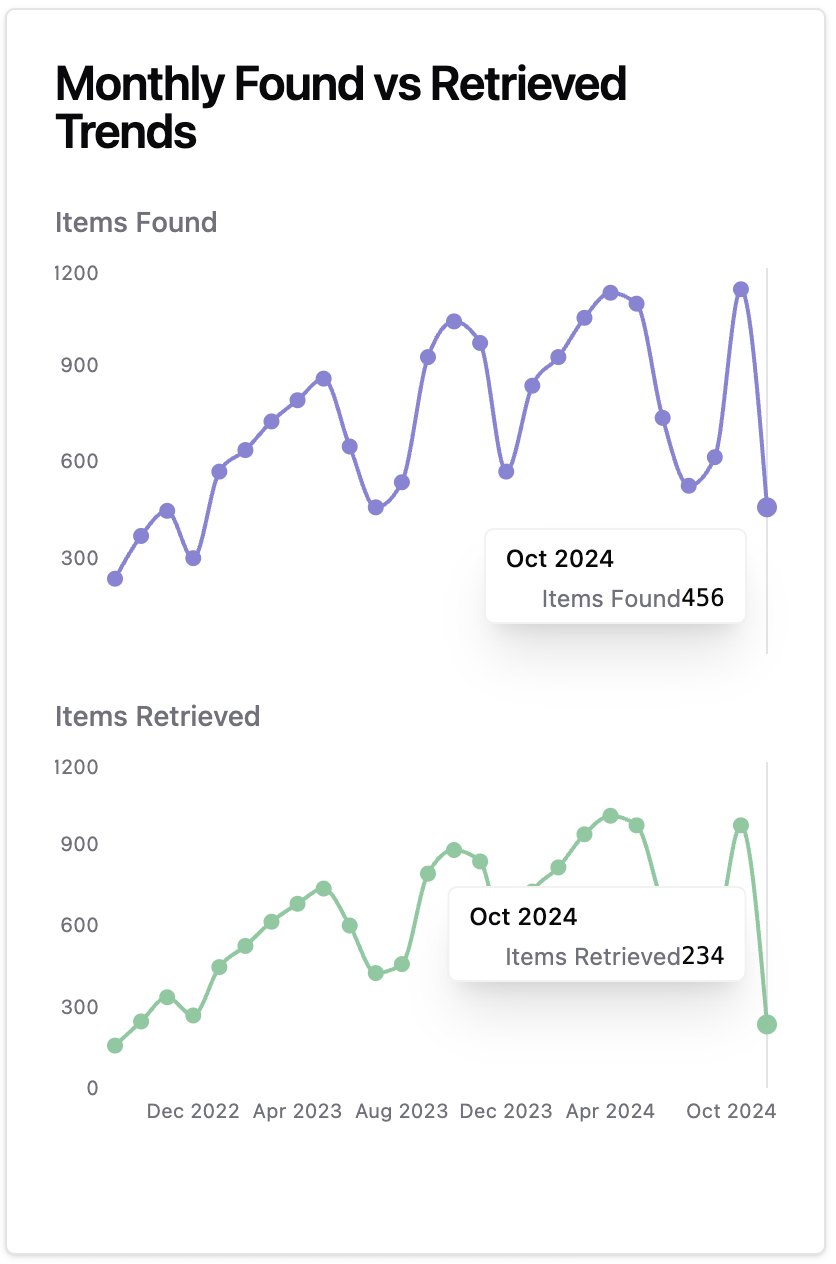
\includegraphics[width=\textwidth]{figs/appendix/web/2C.png}
        \caption{Monthly trends comparing found versus retrieved items, showing system performance with seed data.}
        \label{fig:web_monthly_trends}
    \end{subfigure}
    \caption{Administrative analytics panels showing item distribution, warehouse management, and performance trends.}
    \label{fig:web_analytics_panels}
\end{figure}

\begin{figure}[h]
    \centering
    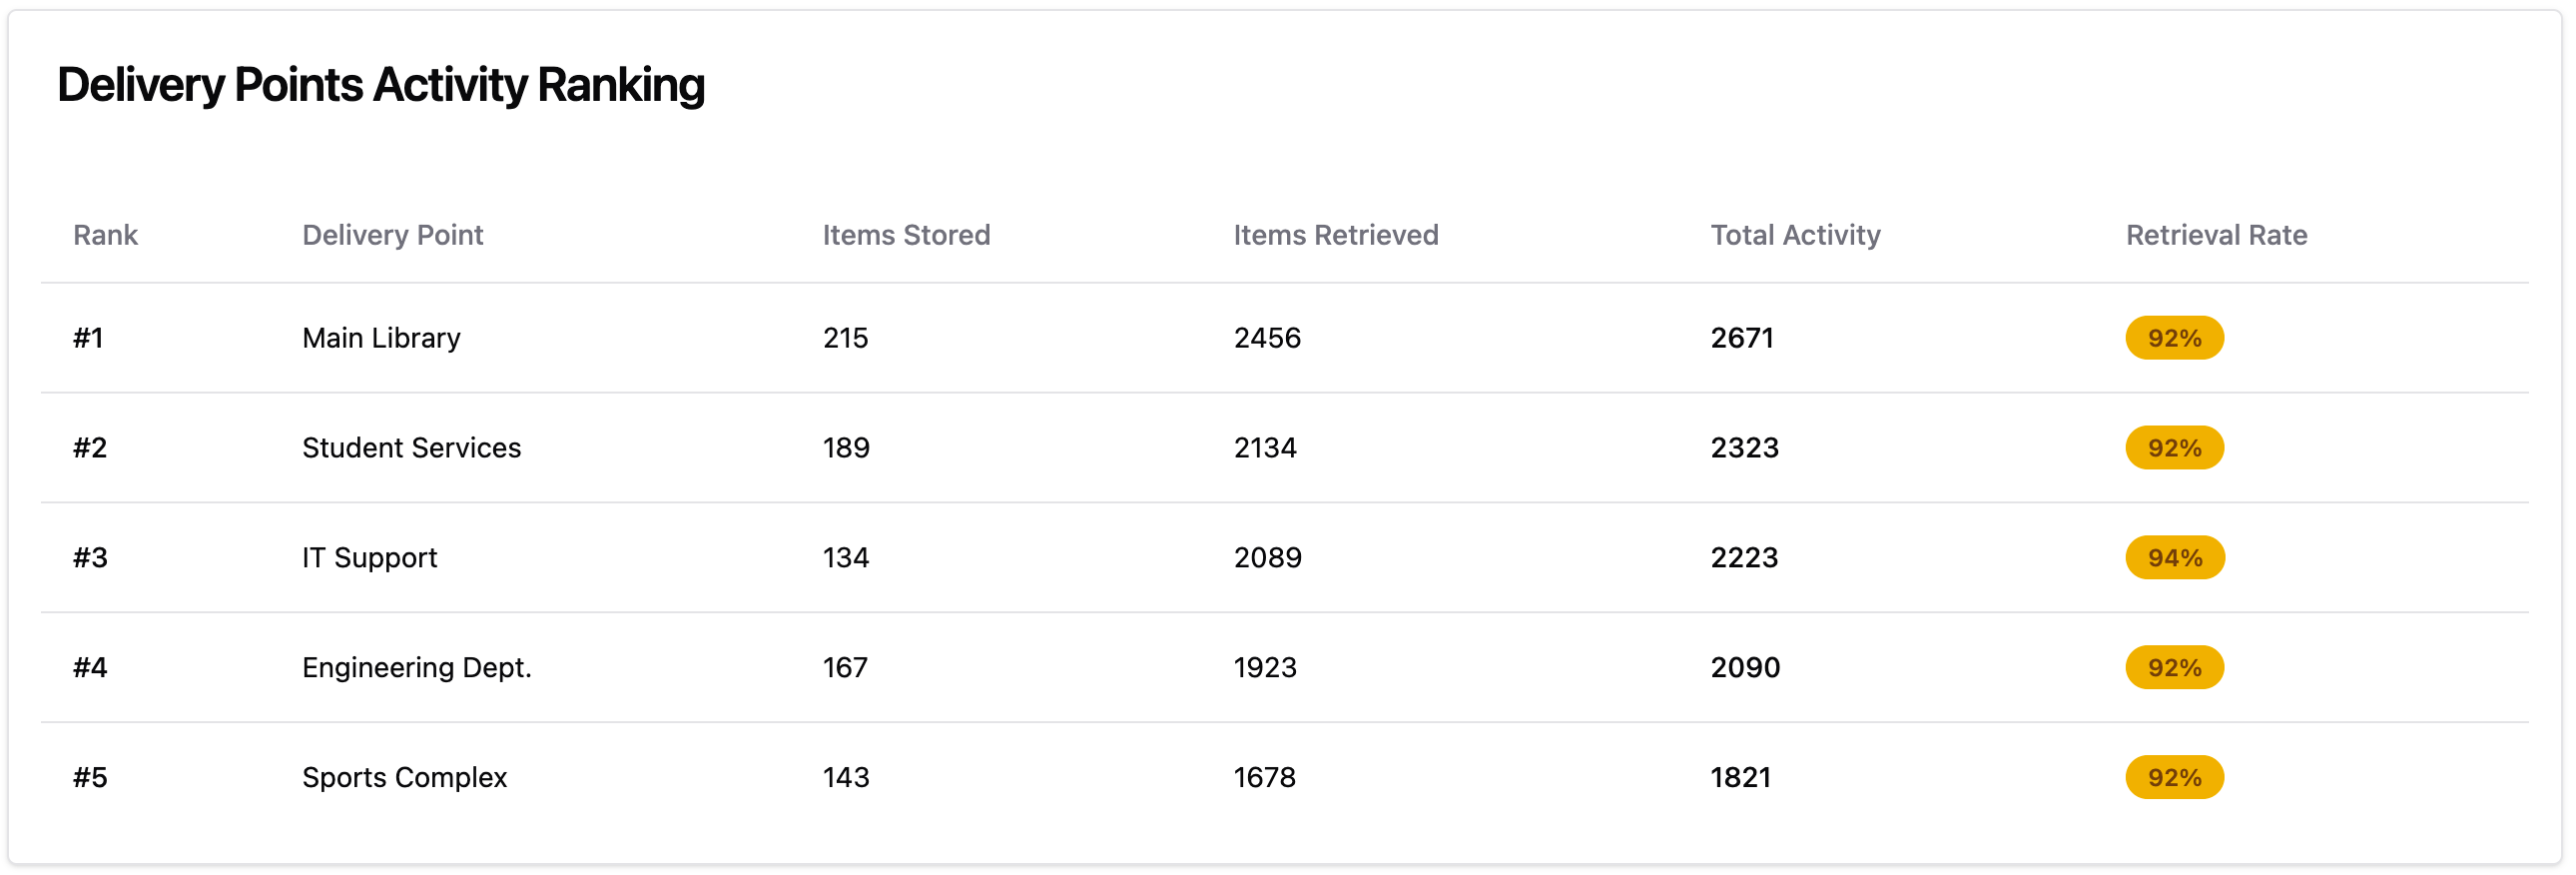
\includegraphics[width=\textwidth]{figs/appendix/web/3.png}
    \caption{Delivery points activity ranking displaying performance metrics for physical collection points.}
    \label{fig:web_delivery_points}
\end{figure}

\begin{figure}[h]
    \centering
    \begin{subfigure}[b]{0.49\textwidth}
        \centering
        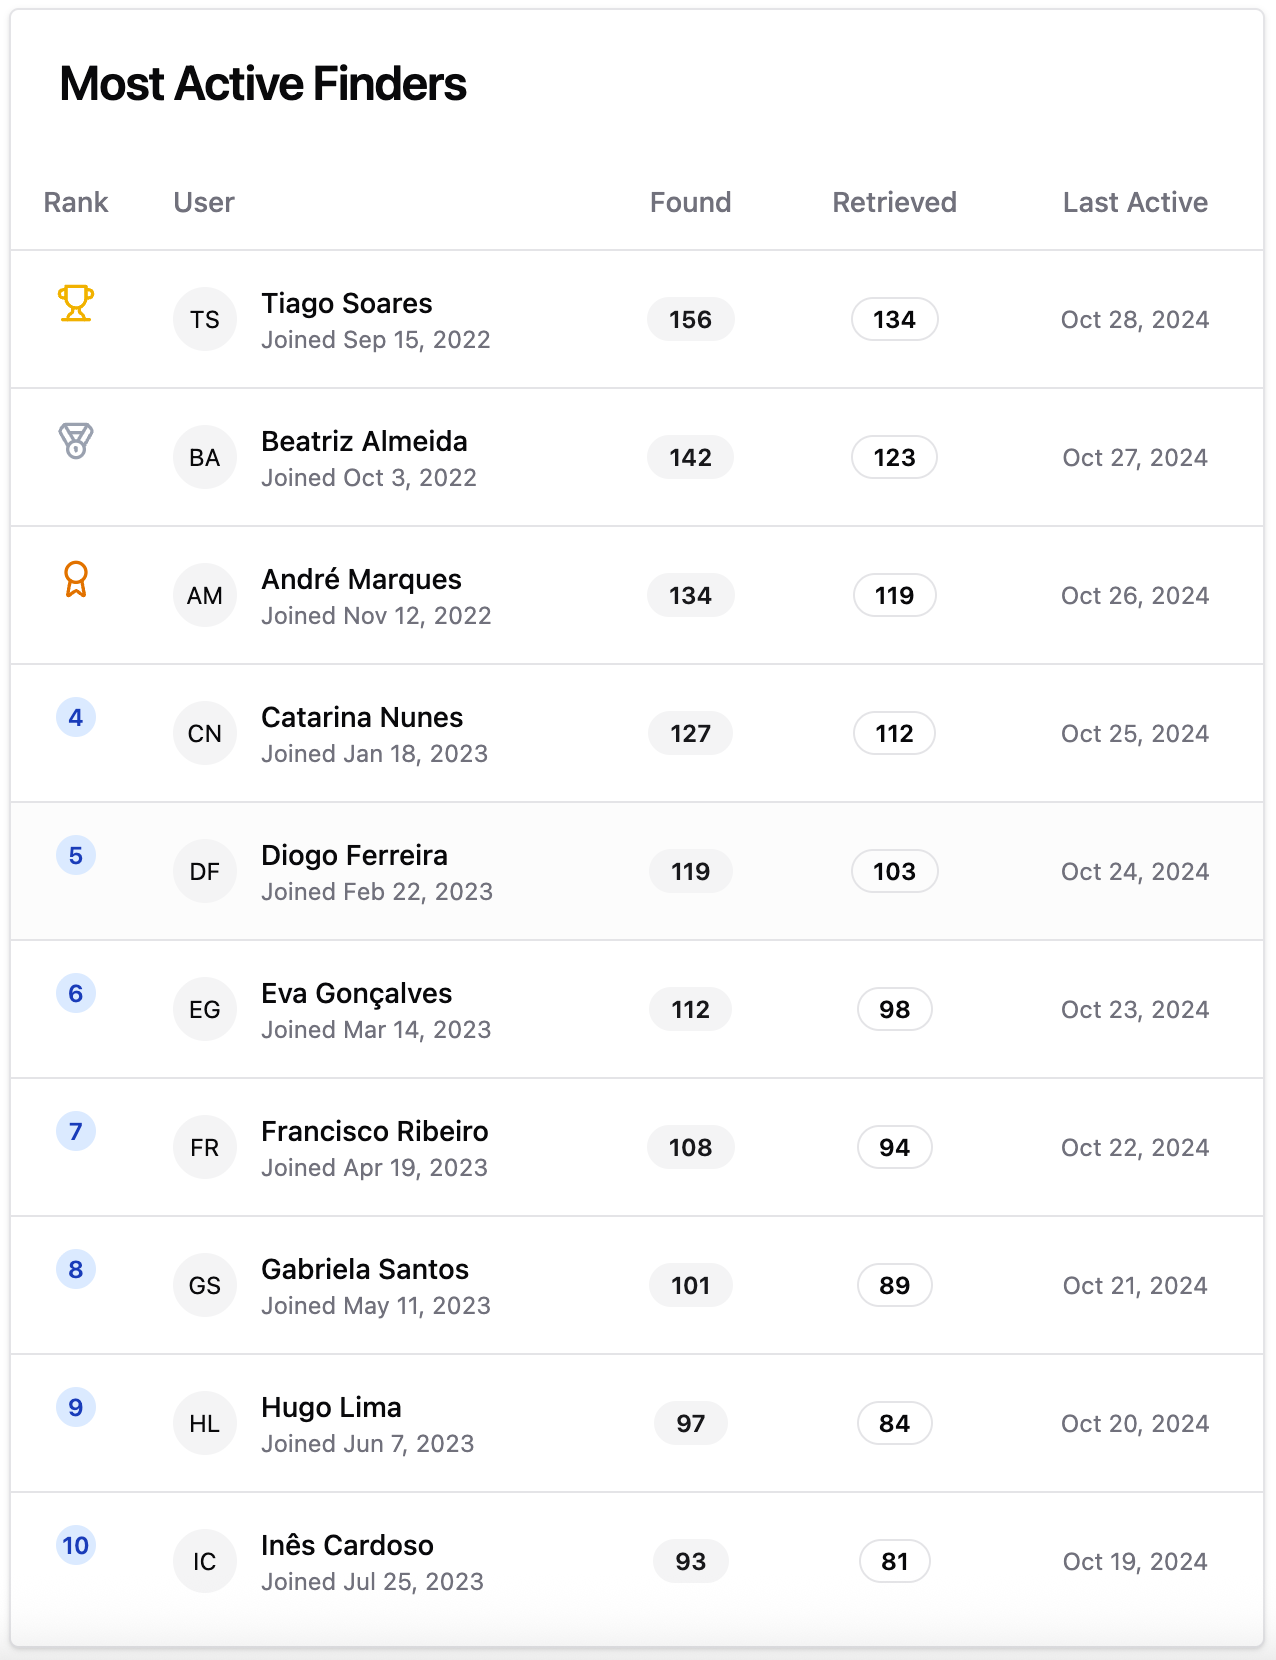
\includegraphics[width=\textwidth]{figs/appendix/web/4A.png}
        \caption{Most active finders leaderboard showcasing community members' contributions.}
        \label{fig:web_active_finders}
    \end{subfigure}
    \hfill
    \begin{subfigure}[b]{0.49\textwidth}
        \centering
        \begin{subfigure}[b]{\textwidth}
            \centering
            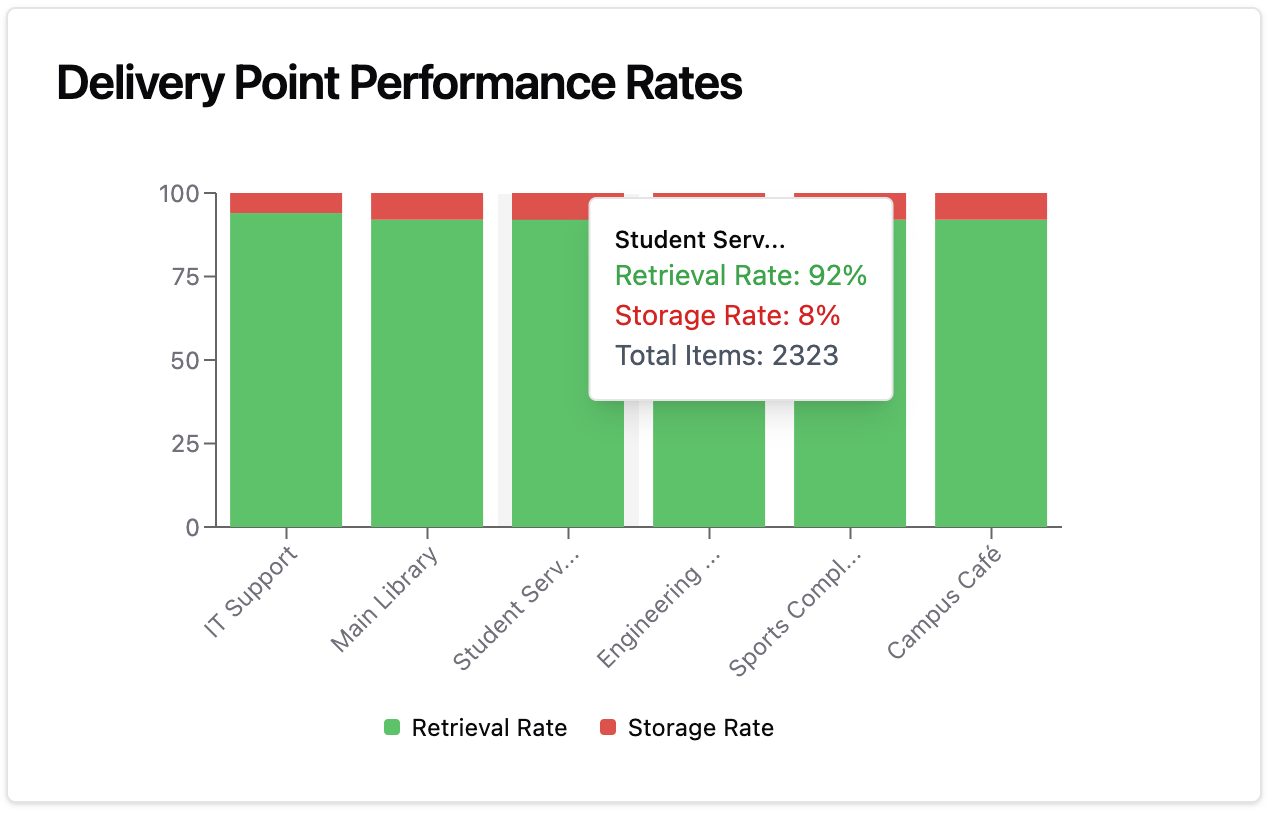
\includegraphics[width=\textwidth]{figs/appendix/web/4B1.png}
            \caption{Delivery point performance rates showing retrieval versus storage distribution across locations.}
            \label{fig:web_performance_rates}
        \end{subfigure}
        \vfill
        \begin{subfigure}[b]{\textwidth}
            \centering
            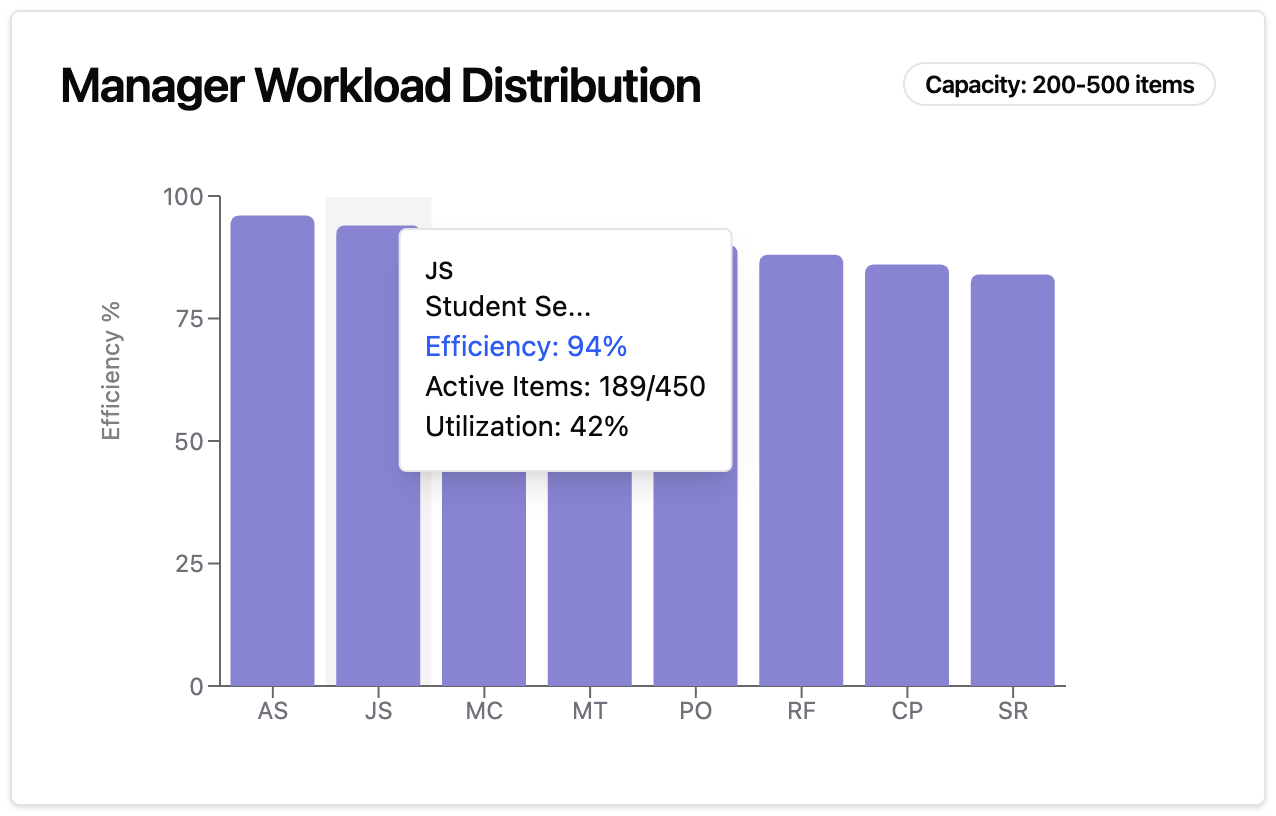
\includegraphics[width=\textwidth]{figs/appendix/web/4B2.png}
            \caption{Manager workload distribution displaying efficiency metrics and capacity utilization across different local managers.}
            \label{fig:web_manager_workload}
        \end{subfigure}
    \end{subfigure}
    \caption{Community engagement and management efficiency panels showing user contributions, delivery point performance, and managerial workload distribution.}
    \label{fig:web_community_management}
\end{figure}

\begin{figure}[h]
    \centering
    \begin{subfigure}[b]{0.49\textwidth}
        \centering
        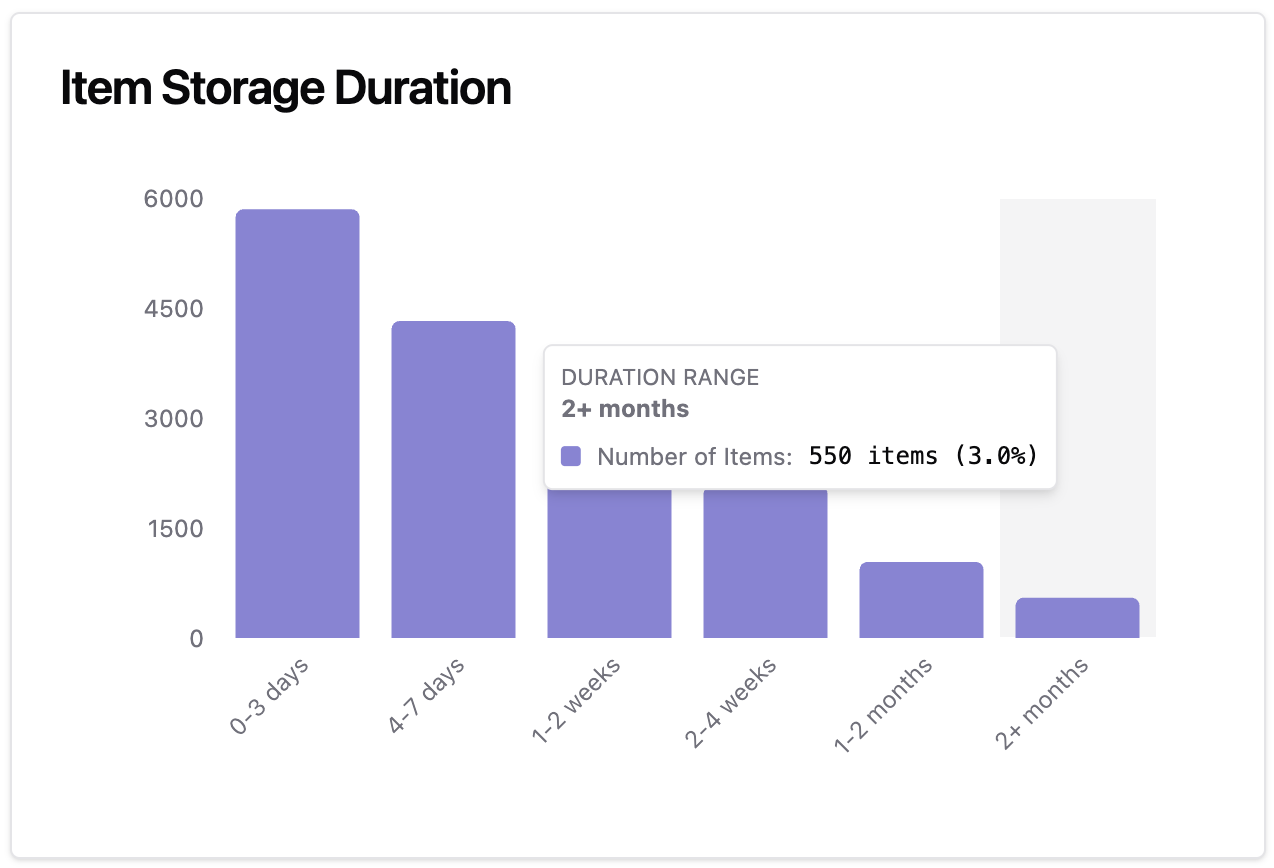
\includegraphics[width=\textwidth]{figs/appendix/web/5A.png}
        \caption{Item storage duration histogram.}
        \label{fig:web_storage_duration}
    \end{subfigure}
    \hfill
    \begin{subfigure}[b]{0.49\textwidth}
        \centering
        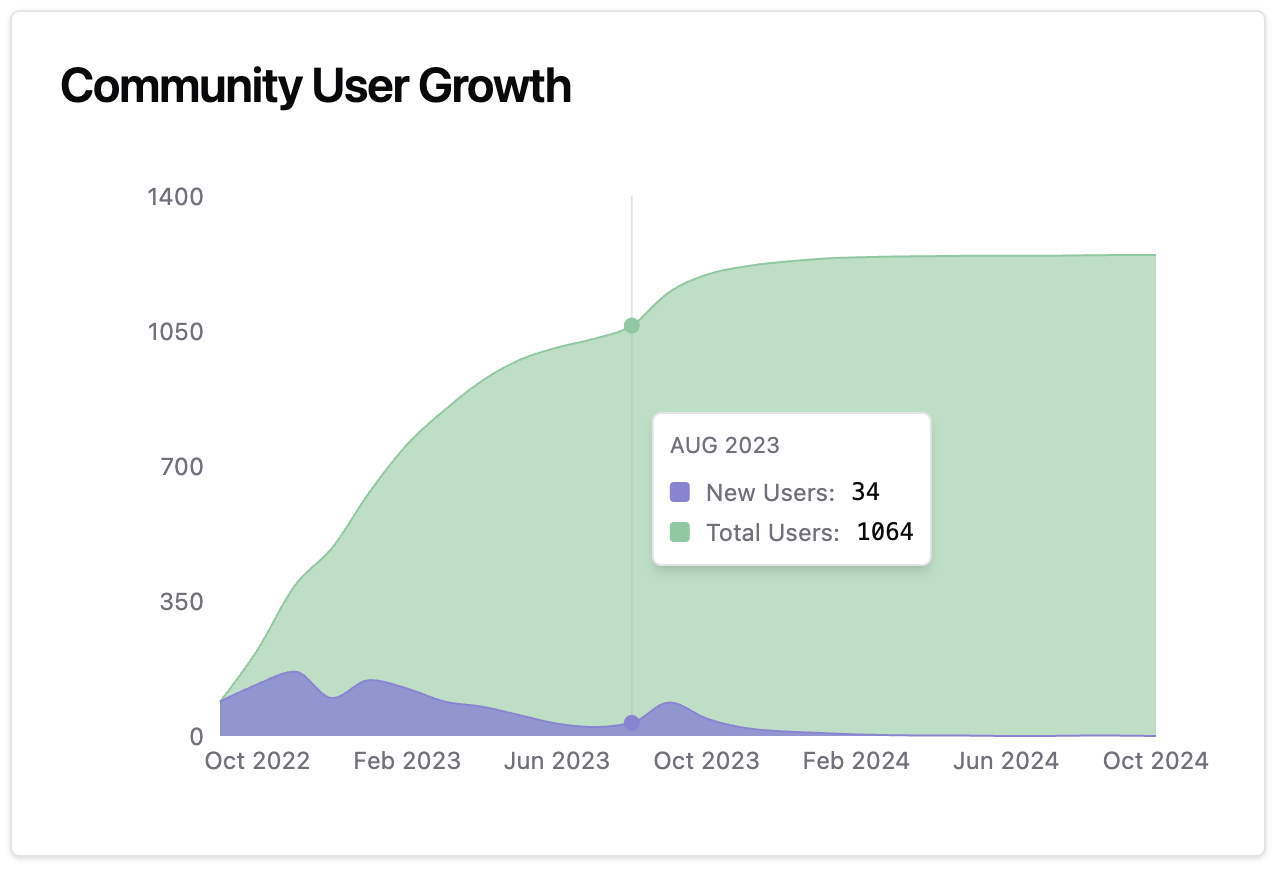
\includegraphics[width=\textwidth]{figs/appendix/web/5B.png}
        \caption{Community user growth area chart tracking system adoption.}
        \label{fig:web_user_growth}
    \end{subfigure}
    \caption{System efficiency and growth analytics showing item retrieval patterns and community expansion over time.}
    \label{fig:web_system_analytics}
\end{figure}

\begin{figure}[h]
    \centering
    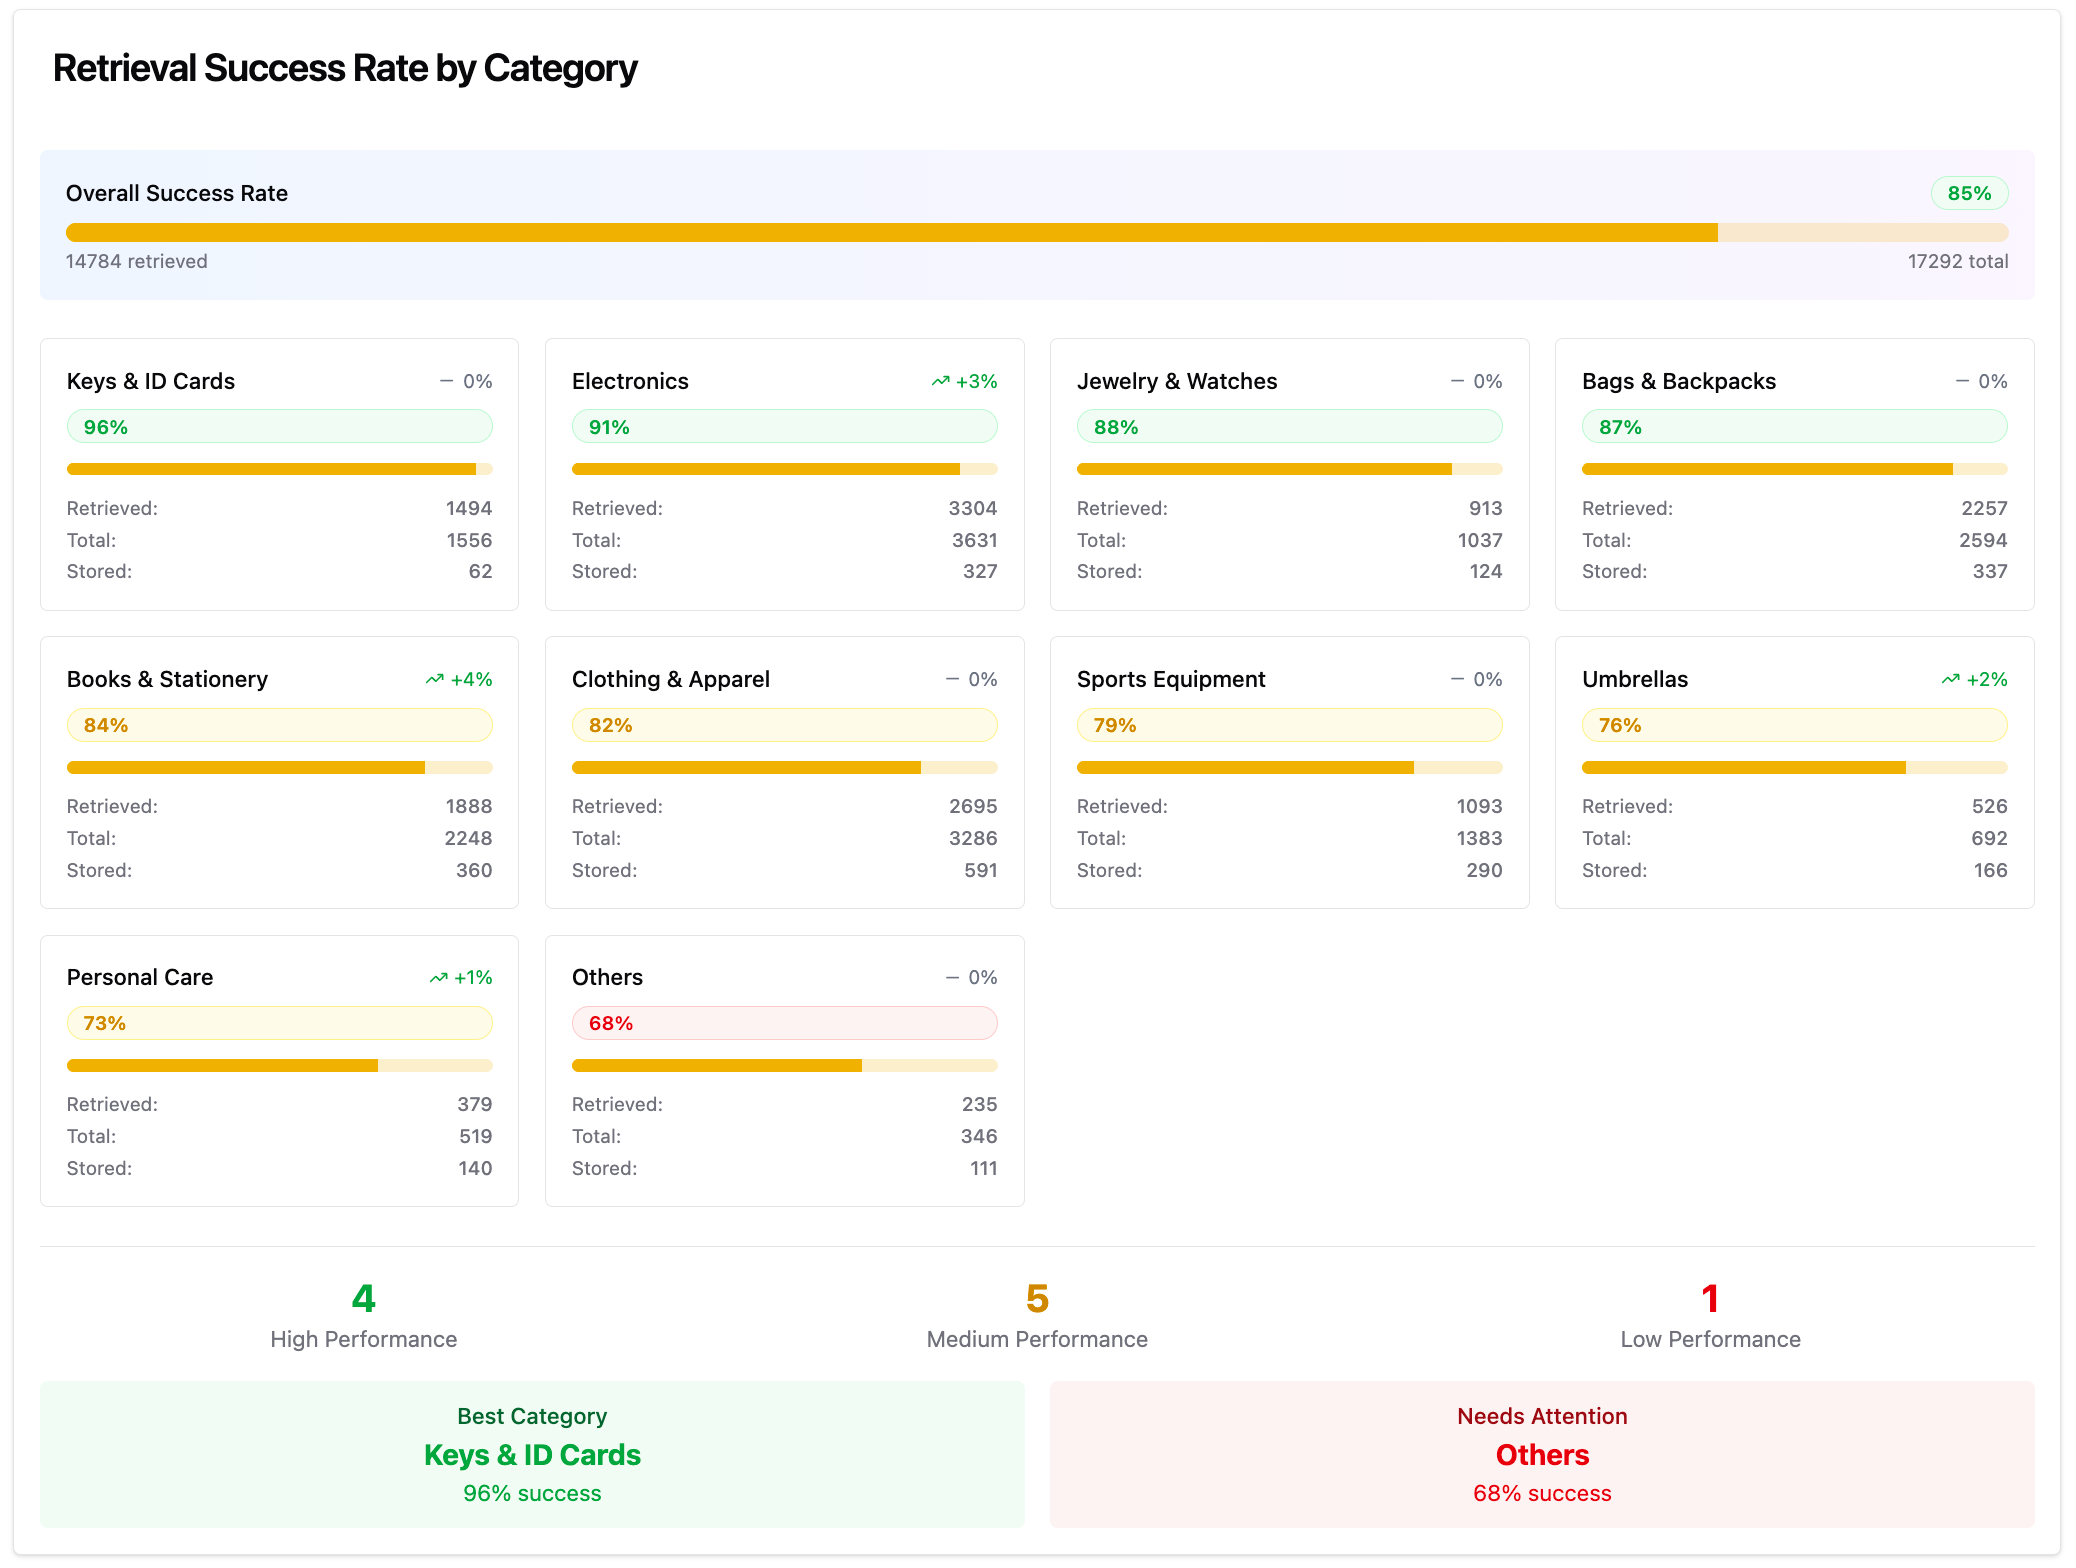
\includegraphics[width=\textwidth]{figs/appendix/web/6.png}
    \caption{Comprehensive retrieval success rate dashboard by category.}
    \label{fig:web_success_rates}
\end{figure}

Dashboard panels allow local managers to monitor performance, track community engagement, and optimize system efficiency across multiple delivery points and user groups. The following sections detail each visualization's purpose and functionality.

\section{System Overview Analytics} \label{section:system_overview}

The system overview dashboard (Figure~\ref{fig:web_dashboard_overview}) presents real-time metrics for monitoring operations. Key performance indicators include total items managed, active managers overseeing delivery points, recent activity patterns, and overall system status. This centralized view allows quick assessment of system health and scale across the university network.

\section{Item Distribution and Warehouse Management} \label{section:item_distribution}

Administrative analytics panels (Figure~\ref{fig:web_analytics_panels}) show patterns across three key dimensions. Category distribution visualization presents the relative proportions of different item types, supporting informed resource allocation decisions based on storage requirements and handling procedures for each category.

Warehouse management view tracks archived items across multiple storage facilities, monitoring current inventory levels and recent archival activity. This information supports storage capacity planning and identifies potential policy review needs for long-term item retention protocols.

Monthly performance trends compare items found against items retrieved over time, allowing administrators to track system effectiveness and identify seasonal variations in lost and found activity patterns. This temporal analysis supports capacity planning and resource allocation during peak periods.

\section{Delivery Point Performance Analysis} \label{section:delivery_points}

Delivery points ranking (Figure~\ref{fig:web_delivery_points}) evaluates collection location performance across campus. The visualization presents activity volumes and retrieval success rates for each delivery point, allowing comparison of effectiveness across different campus locations. This analysis supports resource distribution decisions and identifies best practices for sharing across the delivery point network.

\section{Community Engagement Metrics} \label{section:community_engagement}

Community management panels (Figure~\ref{fig:web_community_management}) track user participation and efficiency across multiple dimensions. The active finders leaderboard identifies community members who contribute most to the lost and found process, recognizing high-performing participants and encouraging continued engagement.

Delivery point performance visualization presents retrieval versus storage ratios through stacked bar representations, with visual indicators showing the proportion of items successfully returned versus those remaining in storage. This analysis helps identify locations requiring improvements.

Manager workload distribution shows capacity utilization and efficiency metrics across different local managers, supporting workload balancing decisions and identification of high-performing managers whose practices can inform training and improvements.

\section{System Efficiency and Growth Patterns} \label{section:efficiency_growth}

Efficiency analytics (Figure~\ref{fig:web_system_analytics}) demonstrate both performance and community adoption trends. The storage duration histogram shows item retrieval patterns over time, indicating matching and notification system effectiveness while highlighting areas for process improvement in long-term case resolution.

Community growth tracking shows user adoption patterns over time, validating system acceptance within the university community and supporting strategic planning for system expansion and resource allocation.

\section{Category-Specific Success Analysis} \label{section:success_analysis}

The retrieval success dashboard (Figure~\ref{fig:web_success_rates}) analyzes performance across item categories, showing overall system effectiveness and category-specific success rates. The visualization identifies which item types achieve the highest retrieval rates and which categories may require improved handling procedures or categorization strategies. This analysis supports improvements and policy development for different item types based on their unique characteristics and retrieval challenges.